\chapter{Formal Verification}

\section{Temporal Logic}
Temporal logic is a rigorous formalism for specifying behaviors of continuous and discrete systems \citep{pnueli1992temporal,manna2012temporal}
provides simple constructs to describe the order in which different “events” in the system
should happen. The basic infrastructure of a formal language provides syntactical operators to handle property verification during time. In literature plenty of formalisms have been proposed, each one specializing either time or application specific features. First part of this chapter aims to analyze some of them starting from their common ancestor, providing also a general comparison.

\subsection{Linear Temporal Logic}
\label{ssec:LTL}

In the Linear Temporal Logic (LTL) time is implicitly represented as an enumerated sequence of reaction steps occurring in a discrete time space. Such temporal logics was developed to check properties in (typically hardware) systems with boolean, discrete-time signals. 
\par LTL with \textit{future} and \textit{past} is defined using the following
syntax:
\begin{center}
$\varphi := \quad p \quad | \quad \neg \varphi \quad | \quad \varphi \vee \varphi \quad | \quad \ocircle  \varphi \quad | \quad \circleddash \varphi \quad | \quad \varphi \; \EuScript{U} \; \varphi |  \quad \varphi \; \EuScript{S} \; \varphi $
\end{center}
where $p$ belongs to a set $P = \{ p_1,\dots,p_n \}$ of propositions indicating values of the corresponding state variable. LTL is interpreted over n-dimensional Boolean $\omega$-sequences of the form $\omega : \mathbb{N} \rightarrow \mathbb{B}^n$. We use $\omega[t]$ to denote the value of a sequence $\omega$ at position $t$ and abuse $p$ to denote the projection of $w$ on variable $p$. The basic future temporal operators are \textit{next} ($\ocircle$), which specifies what should hold in the next step and \textit{until} ($\EuScript{U}$), which requires $\varphi_1$ to hold until $\varphi_2$ becomes true, without bounding the temporal distance to this becoming. From these basic LTL operators one can derive other standard Boolean operators as well as temporal operators such as \textit{eventually} ($\lozenge$) and \textit{always} ($\Box$): 
\begin{center}
$\lozenge \varphi = True \;\; \EuScript{U} \;\; \varphi\quad$and$\quad \Box \varphi = \neg \lozenge \neg \varphi$
\end{center}
Analogously, by means the past temporal operators, is possible to define \textit{eventually in the past}($\mathrlap{\lozenge}{-}$) and \textit{always in the past}($\mathrlap{\Box}{-}$)
\begin{center}
$\mathrlap{\lozenge}{-} \varphi =  True \;\; \EuScript{S}  \;\; \varphi\quad$and$\quad\mathrlap{\Box}{-} \varphi = \neg \mathrlap{\lozenge}{-} \neg \varphi$
\end{center}

The satisfaction relation $(\omega, t) \models \varphi$ indicating that a sequence $\omega$ satisfies $\varphi$ starting from position $t$, is defined inductively as follows:
\begin{equation}
\label{form:LTLop}
\begin{aligned}
 p   & & &(\omega, t) \models \varphi & & &\leftrightarrow & & &p[t] = 1 \\
 not \; \varphi & & &(\omega, t) \models \neg \varphi  & & &\leftrightarrow  & & &(\omega, t) \nvDash \varphi \\
 \varphi_1 \; or \; \varphi_2 & & &(\omega, t) \models \varphi_1 \vee \varphi_2  & & &\leftrightarrow  & & &(\omega, t) \models \varphi_1 \; or \; (\omega, t) \models \varphi_2 \\
 next \; \varphi & & &(\omega, t) \models \ocircle \varphi  & & &\leftrightarrow  & & &(\omega, t+1) \models \varphi \\
 previously \; \varphi & & &(\omega, t) \models \circleddash \varphi  & & &\leftrightarrow  & & &(\omega, t-1) \models \varphi \\
 \varphi_1 \; until \; \varphi_2 & & &(\omega, t) \models \varphi_1 \EuScript{U} \varphi_2  & & &\leftrightarrow  & & & \exists \; t^\prime \in [t, \infty) \; (\omega, t^\prime) \models \varphi_1 \; and \; \forall \; t^{\prime \prime} \in [t, t^\prime), (\omega, t^{\prime \prime}) \models \varphi_2\\
 \varphi_1 \; since \; \varphi_2 & & &(\omega, t) \models \varphi_1 \EuScript{S} \varphi_2  & & &\leftrightarrow  & & & \exists \; t^\prime \in [0, t] \; (\omega, t^\prime) \models \varphi_1 \; and \; \forall \; t^{\prime \prime} \in (t^\prime, t], (\omega, t^{\prime\prime}) \models \varphi_2\\
 \\
 eventually \; \varphi & & &(\omega, t) \models \lozenge \varphi  & & &\leftrightarrow  & & & \exists \; t^\prime \ge t \; (\omega, t^\prime) \models \varphi \\
 always \; \varphi & & &(\omega, t) \models \Box \varphi  & & &\leftrightarrow  & & & \forall \; t^\prime \ge t \; (\omega, t^\prime) \models \varphi
\end{aligned}
\end{equation}

A major difficulty in checking properties expressed in future LTL is due to the \textit{non-causal} definition of the satisfaction relation. In other words, the satisfiability of $\varphi$ at time $t$ may depend on the value of $\omega$ at some future time instant $t^\prime \geq t$. Even worse, some temporal operators refer to future time instants in a \textit{quantified} manner, for example, requiring some $p$ to hold in all future time instants. The satisfiability of such a property may sometime be determined only at infinity, that is, “after” we can be sure
that no instance of $\neg p$ is observed.
\par The causality problem is not present anymore when the recursion goes backward in time, meaning that the satisfaction of a past formula $\varphi$ by a sequence $\omega$ at position $t$ is determined only according to the values of $\omega$ at the interval $[0, t]$. However the futuristic specification keeps a style more natural for humans, for this reason it has been adopted also by industrial specification languages such as PSL (\ref{sec:PSL}).

\paragraph{Evaluation over incomplete behavior}

Monitors do not exploit features of the model representing the system $S$, but rather observe sequences, i.e. model's outputs, as they are produced during simulation. Although the LTL semantic is defined over \textit{complete infinite sequences}, that is for all possible behaviors, is not possible to observe infinite sequence in finite time. Hence, trying to extend the LTL semantic to \textit{incomplete behaviors} represents the hardest challenge in monitoring.
\par At the end of the observation of a certain sequence $\omega$ we can assert one of the following with respect to the property $\varphi$
\begin{enumerate}
\item \textit{$\omega$ satisfies $\varphi$.} Such situation happens, for example, when $\varphi=\lozenge p$ and $p$ occurs in $\omega$.
\item \textit{$\omega$ not satisfies $\varphi$.} For example, when $\varphi=\Box \neg p$ and $p$ occurs in $\omega$.
\item \textit{$\omega$ is undecided.} For example, when $\varphi=\lozenge p$ and $p$ has not yet occurred in $\omega$.
\end{enumerate}
The category "undecided" can be further refined in order to distinguish, for instance, the "not yet violated" ($\varphi=\Box \neg p$) category from the "not yet satisfied" one ($\varphi=\lozenge p$).\\
Even for those cases in which the satisfiability of a property cannot be determined from the observed behavior we would like to give an answer at the end of the sequence. In order to achieve such objective we may consider some LTL sub-classes. One is the bounded-LTL. It provides only \textit{next} as temporal operator, which, in turn, can be used to derive others such as bounded-always and bounded-eventually
\begin{center}
$ \Box_{[0,r]}\varphi = \bigwedge  \limits_{i=0}^{r-1} \ocircle^i \varphi\;\;$ and $\;\;\lozenge_{[0,r]}\varphi = \bigvee  \limits_{i=0}^{r-1} \ocircle^i \varphi$
\end{center}
where $\ocircle^i$ is a shorthand for $\ocircle(\ocircle(\dots\ocircle)p\dots))$. Within this context of timed formulas a global property that has not been violated during the formula's lifetime is considered satisfied. Analogously a property expressing an eventuality not observed during the formula's lifetime is considered violated.

\subsection{Computation Tree Logic}

LTL formulas define properties referring individual executions, or simulations, that is, operators are provided for describing events along a single computation path. 
\par The Computation Tree Logic (CTL) \citep{clarke2008design} extends this concept by expressing formulas with respect to many executions, or simulations, at once. In this sense it belongs to the family of  \textit{branching time logic}, in which operators quantify over the paths that are possible from a given state. The main feature provided by logic such as CTL is the possibility to add temporal connectives to the usual the usual atomic propositional logic formulas.  The temporal connectives are expressions about paths into the future that the state of the system can follow.
\paragraph{} The occurrence of a CTL formula is specified by means the pair \textit{path}, \textit{temporal} quantifiers. The first regards the possible execution paths that the system can follow starting from the current one. The second, instead, relates the occurrences within each single path. 
\par It's clear how LTL logic represents a subset of CTL, in fact an LTL formula can be view as a CTL formula without the specification of the branch quantifier. However, part of the literature uses identify with CTL the sub-logic related to path and with CTL$^*$ the one which unifies both path and temporal quantifiers. According that, LTL and CTL becomes two intersecting set, while CTL$^*$ is the superset containing both. Anyway, for the sake of simplicity, in what follows we will make no difference between CTL and CTL$^*$, using the first in place of the second.

\paragraph{} When evaluating a CTL formula the first member to be considered is the path quantifier. It can be
\begin{description}
\item[A] meaning on \textit{all} the path from the current state, read as "\textit{inevitably}"
\item[E] meaning on \textit{at least one} path from the current state, read as "\textit{possibly}"
\end{description}
Once defined the occurrence among the paths, the second member to consider is the temporal quantifier, i.e.
\begin{description}
\item[X] meaning the next state
\item[G] meaning all the future states, read as "\textit{globally}".
\item[F] meaning in some future state
\item[U] meaning until
\end{description}
Combining the previous operators is possible to generate different types of formulas, suppose that the system is in some state $S$ the formula
\begin{description}
\item[$\varphi$] is true iff it is satisfied by the current state $S$
\item[AX($\varphi$)] is true iff $\varphi$ is true for every immediate successor of state $S$
\item[AG($\varphi$)] is true iff $\varphi$ is true for every successor to state $S$, including $S$. That is, $\varphi$ is true for all states on all paths into the future from $S$, i.e. the subtree originating from $S$
\item[AF($\varphi$)] is true iff on all paths into the future from $S$, there is a state where $\varphi$ holds
\item[A [$\varphi_1$ U $\varphi_2$]] is true iff all paths starting in state $S$ satisfy $\varphi_1$ until the reach a state in which $\varphi_2$ holds
\\
\item[EX($\varphi$)] is true iff $\varphi$ is true for at least one immediate successor to state $S$
\item[EG($\varphi$)]  if true iff there is a path from $S$ into the future for which $\varphi$ holds for every state on the path, including $S$
\item[EF($\varphi$)] is true iff there exists a path into the future from $S$ on which there is a state where $\varphi$ holds
\item[E [$\varphi_1$ U $\varphi_2$]] is true iff there exists a path starting in state $S$ that satisfies $\varphi_1$ until reaching a state in which $\varphi_2$ holds
\end{description}
A graphical representation of the above formulas is shown in Figure \ref{fig:ctl}
\begin{figure}[!h]
	\centering 
     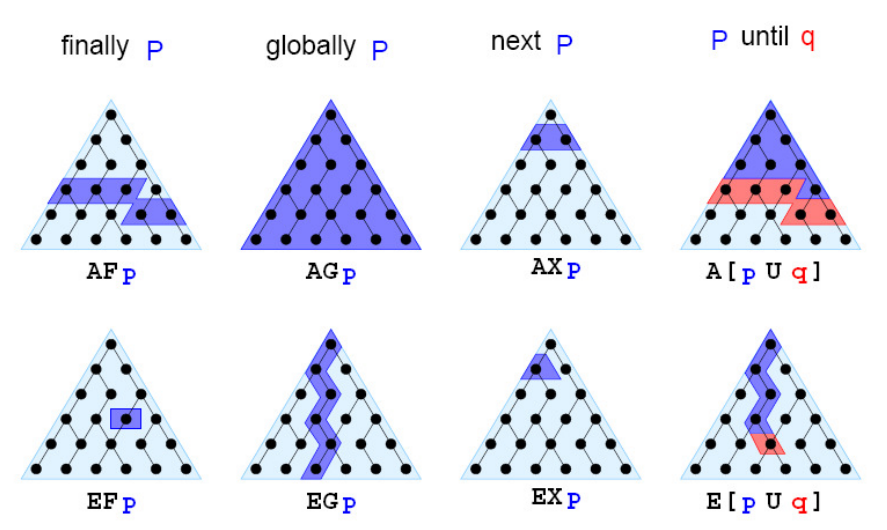
\includegraphics[width=.9\textwidth]{Figs/ctl.PNG} 
     \caption{CTL formulas} 
     \label{fig:ctl} 
\end{figure} 

\noindent
A subset Computation Tree Logic is supported for verification in UPPAAL, which is an integrated tool environment for modeling, validation and verification of real-time systems modeled as networks of timed automata \citep{uppaal}.

\subsection{Property Specification Language}
\label{sec:PSL}

The Property Specification Language (PSL) \citep{eisner2007practical} is a formal language for specification of electronic system behavior, compatible with multiple electronic system design languages. In 2005 it became an IEEE standard \citep{ieee2005ieee}. PSL was designed to be mathematically rigorous, with the result that a PSL specification is both precise and automatically verifiable. Thus, a hardware specification written in PSL is machine readable and can be used as input to verification tools.

\paragraph{} Being a specification language whose targets is the hardware, signals in PSL are used as stream of bits having a fixed length, and , for the same reason, time is meant as a sequences of \textit{clock-cycles}. The structure of PSL is based on four layers
\begin{enumerate}[label={--}]
\item The \textit{boolean layer} is composed of Boolean expressions. PSL interprets a high signal as true, and a low signal as false, independent of whether the signal is active-high or active-low. Operations of the Boolean layer are expressed through the supported hardware specification languages such as Verilog, VHDL and so on.
\item The \textit{temporal layer} consists of temporal properties which describe the relationships between Boolean expressions over time. The semantic of temporal operators is quite similar to the LTL ones.
\item The \textit{verification layer} consists of directives which describe how the temporal properties should be used by verification tools. For instance, is possible to define verification or assumption directives, which tells the tools to verify the value of some property or specify coverage criteria. The verification layer also provides a means to group PSL statements into \textit{verification units}.
\item The \textit{modeling layer} provides a means to model behavior of design inputs, and to declare and give behavior to auxiliary signals and variables
\end{enumerate}

While the Boolean layer consists of Boolean expressions that hold or do not hold at a given cycle, the temporal layer provides a way to describe relationships between Boolean expressions over time. A PSL assertion typically looks in only one direction – forwards from the first cycle. Thus, the simplest PSL assertion \textbf{assert a;} states that signal \textbf{a} should hold at the very first cycle. 
\noindent
\\
The PSL temporal operators are the following
\begin{description}
\item[always ($p$)] meaning that property $p$ must \textit{globally} hold
\item[never ($p$)] meaning that property $p$ must \textit{never} hold
\item[next ($p$)] will hold if its operand, $p$, holds at the next clock-cycle. Variations on the next operator allows to specify ranges of future cycles, i.e. a  \textbf{next a[i:j]($p$)} property holds if its operand holds in all of the cycles from the $i^{th}$ next cycle through the $j^{th}$ next cycle, inclusive.
\item[$p$ until $q$] provides a way to move forward, meaning that property $p$ must hold \textit{until} $q$ hold. In order to include the cycle in which $q$ holds the \textbf{until\_} is normally used.
\item[$p$ before $q$] is dual to \textbf{until} and requires that its first operand happen strictly before
its second. Even for this case in order to include the cycle in which $q$ holds, namely is allowed an overlap between left and right sides, the \textbf{before\_} is used.
\item[eventually!($p$)] allows you to specify that $p$ must occur in the future without saying exactly when.
\end{description}
A good feature of PSL is that it let user choose how the formulas are evaluated in cases of incomplete behavior. Such problem, already discussed in section \ref{ssec:LTL}, rises whenever the simulation, or execution, time is not enough to determine the satisfiability of a formula. PSL handles this providing the possibility to define the strength of an operator, therefore operators can be claimed as \textit{strong}  or \textit{weak} depending on the addition of an exclamation mark (\textbf{!}) to their names. Formulas with strong operators, marked with (\textbf{!}), are considered satisfied if the simulation time is \textit{enough}  and the property holds, for instance \textbf{next![n]} indicate that at least $n$ cycles are needed. Some operators, anyway ,constitutes an exception since they are only allowed in their weak (\textbf{always}, \textbf{never}) or strong (\textbf{eventually!}) versions. Moreover, PSL offers many other versions of \textbf{next} associated with occurrence of events rather than cycles, for further details refer \citep{eisner2007practical}.

\subsection{Signal Temporal Logic}
\label{sec:STL}

Signal Temporal Logic (STL) \citep{maler2004monitoring} is a temporal logic for specifying properties on \textit{dense-time real-valued signals}. Such a logic is particularly useful in domains like \textit{control systems}, where continuous variables are used to model the physical plant	under control. The natural models for such systems are differential equations, for purely continuous systems, or hybrid systems when the dynamics is mixed and contains mode switching, saturation, etc. Before going into details of STL is useful to analyze it's direct ancestor MITL.

\paragraph{Metric Interval Temporal Logic} The \textit{real-time temporal logic} MITL \citep{alur1996benefits} allows reasoning over Boolean signals over dense-time domains. Formally, signals are functions of the form $s: \mathbb{T} \rightarrow \mathbb{B}$, where the time domain $\mathbb{T}$ is the set of non-negative real numbers $\mathbb{R}_+$.
\par We consider the logic MITL$_{[a,b]}$ as a fragment of MITL, such that all temporal modalities are restricted to intervals of the form [$a, b$] with $0 \leq a < b$ and $a, b \in \mathbb{Q}+$. Similarly to \ref{ssec:LTL}, the use of bounded temporal properties is justified by the nature of monitoring where the behavior of a system is observed for a finite time interval. The basic formulas of MITL$_{[a,b]}$ are defined by the grammar
\begin{center}
$\varphi := \quad p \quad | \quad \neg \varphi \quad | \quad \varphi \vee \varphi \quad | \quad \varphi_1 \; \EuScript{U}_{[a,b]} \; \varphi_2 $
\end{center}
From basic MITL[a,b] operators one can derive other standard Boolean and temporal operators, in particular the time-constrained eventually and always operators:
\begin{align*}
\lozenge_{[a,b]} \varphi &= True \; \EuScript{U}_{[a,b]} \; \varphi \\
\Box_{[a,b]} \varphi &= \neg \lozenge_{[a,b]} \neg \varphi 
\end{align*}
The semantic of the unbounded operators is equivalent to the one provided for LTL (\ref{form:LTLop}), while the introduction of the time window modifies \textit{until}, \textit{eventually} and \textit{always} as follow
\begin{align*}
(s, t) \models \varphi_1 \EuScript{U}_{[a,b]} \varphi_2 &\leftrightarrow \exists \; t^\prime \in [t+a, t+b] \; (s, t^\prime) \models \varphi_2 \; and \; \forall \; t^{\prime \prime} \in [t, t^\prime], (s, t^{\prime \prime}) \models \varphi_1 \\
(s, t) \models \lozenge_{[a,b]} \varphi &\leftrightarrow \exists \; t^\prime \in [t+a, t+b], (s, t^\prime) \models \varphi \\
(s, t) \models \Box_{[a,b]} \varphi &\leftrightarrow \forall \; t^\prime \in [t+a, t+b], (s, t^\prime) \models \varphi
\end{align*}
By using bounded operators we avoid the problems related to the ambiguity
of $\models$ when applied to finite signals or sequences. Nevertheless, even for MITL$_{[a,b]}$ certain signals are too short to determine satisfaction of the formula, for example the property $\Box_{[a,b]}\lozenge_{[c,d]}p$ cannot be evaluated on signals shorter than $b + d$.

\paragraph{} We can now extend our semantic domain and logic to real-valued signals. While Boolean signals of finite variability admit a finite representation, this is typically not the case for real-valued signals which are often represented via sampling, that is a sequence
of time stamped values of the form $(t, s[t])$. Although the semantics of the logic is defined in terms of the mathematical objects, for signals of the from $s : \mathbb{T} \rightarrow \mathbb{R}^n$ is not possible to ignore issues related to their effective representation based on the output of some numerical simulator. For this reason STL does not directly cope with continuous signal, but rather via a set of abstraction of the form $\mu : \mathbb{R}^n \rightarrow \mathbb{B}$. Typically $\mu$ partitions the continuous state-space according to the satisfaction of some inequality constraints on the real variables. As long as $\mu(s[t])$ remains constant we do not really care about the exact value of $s[t]$. However, in order to evaluate formulas we need the sampling to be sufficiently dense so that all such transitions can be detected when they happen. From now on we assume that we deal with signals that are well-behaving with respect to every $\mu$, that is, every change in $\mu(s)$ is detected in the sense that every point $t$ such that $\displaystyle{\mu(s[t]) \neq \; \lim_{t^\prime\to t} \; \mu(s[t]^\prime)}$ is included in the sampling.

\paragraph{} We can define an STL formula as a MITL$_{[a,b]}$ formula over the atomic propositions $\mu_1(s(t)),\dots,\mu_m(s(t))$, where each $\mu_i$ is a predicate of the form $\mu_i:\mathbb{R}^n\rightarrow\mathbb{B}$. The monitoring process for STL formula decomposes hence into two phases, in which the first is always the construction of a Boolean “filter” for every $\mu_i \in U = \{\mu_1 , \dots ,\mu_m \}$, which transforms $s$ into a Boolean signal $p_i = \mu_i(s)$.

\subsection{Summary}

\section{Patterns Identification}

The drawback to using temporal logics for property specification is their steep learning curve for industrial practitioners. Consequently, designers and developers will be less likely to use verification tools if they must devote large amounts of time to learning a specification language. Even with significant expertise, dealing with the complexity of such a specification could be daunting. As many other disciplines, like \textit{software engineering}, complexity in this context is addressed through the definition and use of common \textit{patterns}. Patterns are meant as a further levels of abstraction, parameterizable and often formalism-independent. 

\subsection{Property Specification Patterns}

Property specification patterns \citep{dwyer1998property} describe commonly observed requirements in a generalized manner. Observing the several formalisms introduced before is possible to notice how there are two basic parts of properties that commonly occur. The first tells when the property should hold, and the second tells what condition should be satisfied during this time. Precisely each formula consists of two pieces: a \textit{scope} and a \textit{pattern}. The scopes defines \textit{when} a particular property should hold during the simulation, the pattern, instead, the condition that must be satisfied. The are five basic kinds of scopes that can be recognized,
\begin{description}
\item[Globally] meaning the entire simulation
\item[Before R] meaning the entire execution up to the occurrence of \textbf{R}
\item[After Q] meaning the entire execution from the occurrence of \textbf{Q}
\item[Between Q and R] any piece of simulation from the occurrence of Q and the occurrence of \textbf{R}
\item[After Q until R] like above but holds even if \textbf{R} does not occur
\end{description}
\begin{figure}[!h]
	\centering 
     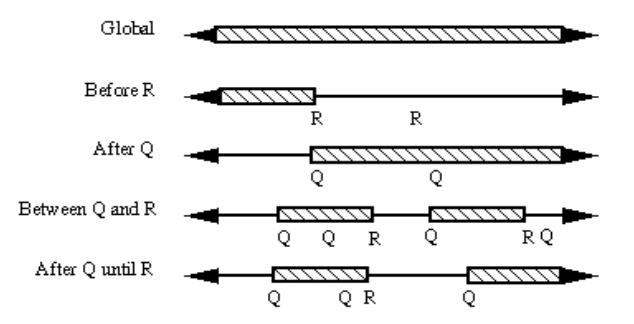
\includegraphics[width=.7\textwidth]{Figs/scopes.PNG} 
     \caption{Property Scopes} 
     \label{fig:scopes} 
\end{figure} 
Figure \ref{fig:scopes} illustrates the portions of an execution that are designed by the different kind of scopes.
\par Patterns are organized in a hierarchical manner based on their semantic. A the first level they are divided by \textit{occurrence} and \textit{order}. Firsts are used to express requirements related to the existence (or lack of existence) of certain states/events during well-defined regions of system execution, while seconds are used to express requirements related to pairs of states/events during well-defined regions of system execution. For both categories regions are defined using \textit{scopes}. In the class of Occurrence patterns we find
\begin{description}
\item[$P$ is false (Absence)] to describe a portion of a system's execution that is free of certain events or states.
\item[$P$ is true (Universality)] to describe a portion of a system's execution which contains only states that have a desired property.
\item[$P$ becomes true (Existence)] to describe a portion of a system's execution that contains an instance of certain events or states.
\item[$P$ occur at most $N$ times (Bounded Existence)] to describe a portion of a system's execution that contains at most a specified number of instances of a designated state transition or event.
\end{description}
while Order patterns are
\begin{description}
\item[$S$ precedes $P$ (Precedence)] to describe relationships between a pair of events/states where the occurrence of the first is a necessary pre-condition for an occurrence of the second.
\item[$S$ responds to $P$ (Response)] to describe cause-effect relationships between a pair of events/states.
\item[$Q_1\dots Q_n$ precedes $P_1\dots P_n$ (Precedence Chain)] to describe a relationship between a sequence of events/states and a sequence of events/states. The occurrence of sequence $P_1\dots P_n$ must be preceded by an occurrence of the the sequence $Q_1\dots Q_n$.
\item[$P_1\dots P_n$ responds $Q_1\dots Q_n$ (Response chain)] to describe a relationship between stimulus events and a sequence of response events. The occurrence of the stimulus $P_1\dots P_n$ must be followed by an occurrence of the sequence $Q_1\dots Q_n$.
\end{description}
Clearly patterns are not unique in the sense that one can be achieved by combination of some others. The Absence, for instance, is dual to Existence, while Precedence is converse to Response. This redundancy does not represents an issue but rather extends the usability of those patterns even in formalisms that not provide complete support for all scope operators. Figure \ref{fig:phierarchy} provides an overview of patterns classification.
\begin{figure}[!h]
	\centering 
     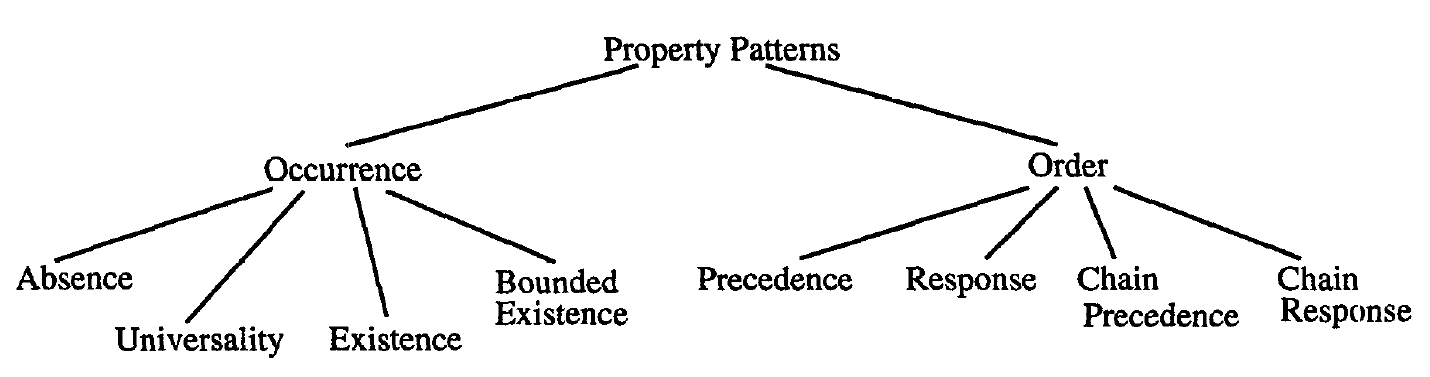
\includegraphics[width=.9\textwidth]{Figs/hierarchy.PNG} 
     \caption{Pattern Hierarchy} 
     \label{fig:phierarchy} 
\end{figure} 

Being each pattern defined over a scope, the number of possible achievable combinations corresponds to the dimension of the set generated by the product of scope and pattern sets. Each combination could be mapped in a specific requirements, therefore it can be independently translated in a chosen formalism. For the sake of briefness we show the complete LTL an CTL formalization for just a pattern, and refer \citep{specpatterns} for an exhaustive list. 
\par Before describe the pattern lets define the \textit{weak until} operator $\EuScript{W}$ which is used make less verbose the expression of some formulas.
\begin{center}
\begin{tabular}{ll}
LTL: &$P \;\EuScript{W}\; Q = P \;\EuScript{U} \; (Q\; |\; \Box\:P) $ \\
CTL: &$P$ \textbf{W} $Q = \neg$E ($\neg Q$ \textbf{U} ($\neg P$ $\&$ $\neg Q$))
\end{tabular}
\end{center}
\paragraph{Universality} \textbf{$P$ is true}\noindent\\
\begin{tabular}{ll}
\textit{Scope} & \textit{LTL} \\
Globally & $ \Box\;P$ \\ 
Before $R$ & $A\;R\rightarrow(P\;\EuScript{U}\;R)$\\
  After $Q$ & $ \Box\;R\rightarrow(Q\rightarrow \Box\; P)$	\\
Between $R$ and $Q$ & $ \Box\;((Q\; \&\; \neg R\; \&\; \lozenge\:R)\rightarrow(P\;\EuScript{U}\;R))$	\\
\end{tabular}
\\
\\
\begin{tabular}{ll}
\textit{Scope} & \textit{CTL} \\
Globally & \textbf{AG}($P$) \\ 
Before $R$ & \textbf{A}(($P$ | \textbf{AG}($\neg R$)) \textbf{W} $R$)\\
After $Q$ & \textbf{AG}($Q \rightarrow $ \textbf{AG}($P$))	\\
Between $R$ and $Q$ & \textbf{AG}($Q\;\&\;\neg R \rightarrow$ \textbf{A}(($P$ | \textbf{AG}($\neg R$)) \textbf{W} $R$	\\
After $Q$ unitl $R$ & \textbf{AG}($Q\;\&\;\neg R \rightarrow$ \textbf{A}($P$ \textbf{W} $R$))
\end{tabular}

\subsection{Domain Patterns}
\label{ssec:dompatterns}

When dealing with complex systems quite often the requirements analysis is performed at different levels of abstraction. As result the complete specification is provided by many requirements documents, in which requirements of a certain level are grouped according to derivation from a \textit{parent requirement} belonging to an higher level. 
\par A typical scenario for control systems is that high-level requirements focus all those properties specific of that application domain. Examples are the so called \textit{performance requirements}, which assess features of the system response over time. Since they refer properties having a well-known mathematical representation such kind of requirements in turn are prone to have a parameterizable definition. In other words they are suitable to become domain specific patterns.
\par Two typical performance requirements expressed in natural language are the following
\begin{quote}
\begin{enumerate}
\label{en:ptreq}
\item \textit{The Driver System (DRV) shall accelerate the motor from zero to $x_1$ rpm in less than $t_1$ sec, with an overshoot of less than $x_2$ rpm  and a time to settle to within $\pm x_3$ rpm of $x_4$ rpm of less than $t_2$ ms with a system inertia less than or equal to $S_{In}$}
\item \textit{The Driver System (DRV) shall decelerate the motor from $x_1$ to zero rpm in less than $t_1$ sec, with an undershoot of less than $x_2$ rpm and a time to settle to within $\pm x_3$ rpm of  zero rpm of less than $t_2$ ms with a system inertia less than or equal to $S_{In}$}
\end{enumerate}
\end{quote} 
An informal definition of the addressed requirements is the following
\begin{description}
\item[Rise(Fall)-time] is the amount of time it takes for a signal to rise (fall) from an initial value to another value some distance from an expected steady state value in response to a step input  (Fig.\ref{fig:risetime})
\item[Overshoot (Undershoot)] is a quantity that defines how much a signal goes beyond an expected steady state value in response to a step input (Fig.\ref{fig:overshoot})
\item[Settling-Time] is the time it takes a signal to reach and remain within a band around a steady state value in response to a step input (Fig.\ref{fig:settime})
\end{description}
\begin{figure}[h]
    \centering
    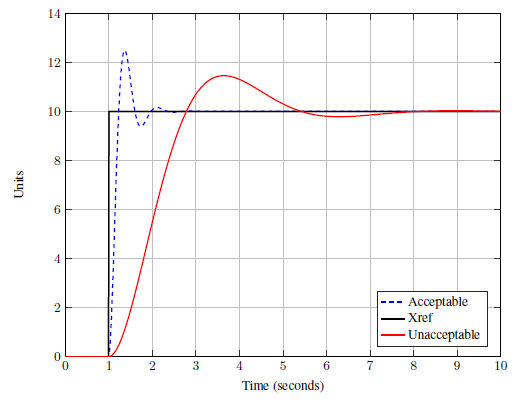
\includegraphics[width=.6\textwidth]{Figs/risetime.PNG}
    \caption{Rise Time}
    \label{fig:risetime}
\end{figure}
\begin{figure}[h]
    \centering
    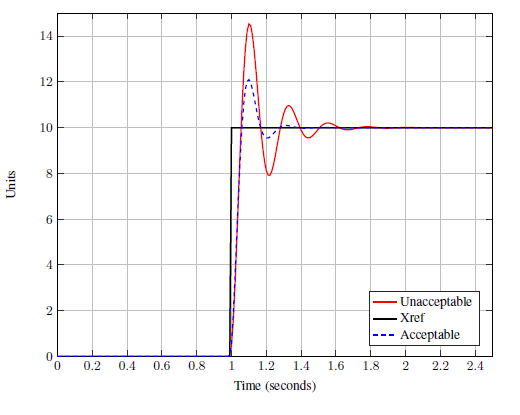
\includegraphics[width=.6\textwidth]{Figs/overshoot.PNG}
    \caption{Overshoot}
    \label{fig:overshoot}
\end{figure}
\begin{figure}[ht]
    \centering
    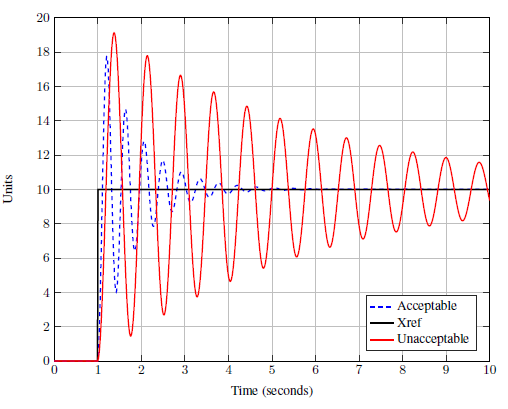
\includegraphics[width=.6\textwidth]{Figs/settime.PNG}
    \caption{Settling Time}
    \label{fig:settime}
\end{figure}
\paragraph{} In \citep{kapinski2016st} J.Kapinski et al provided an STL formalization for above property. Since all of them are defined in response to an asynchronous step input they extended the STL language to provide the operator
\begin{center}
$step(x,a) \triangleq x(t+\epsilon) - x(t) > a$
\end{center}
where $a$ is the step amplitude and $\epsilon$ corresponds to the smallest time variation following $t$. 
In the case the formula has to be verified by a discrete time monitors $\epsilon$ is equal to the sample time.
\par In STL, timed formulas can be nested such as, for example,
\begin{center}
$\lozenge_{[0, T]}(\textbf{q} \wedge \Box_{[a,b]} \textbf{p})$
\end{center}
The proposition $\textbf{p}$ is nested one level deeper than proposition $\textbf{q}$. The meaning is that there has to be one time instant $t$ in $[0,T]$ (the outer Eventually condition) such that $\textbf{q}$ is satisfied in $t$ and for all the system evolutions starting from time $t$, the condition $\textbf{p}$ is verified at some time between $t + a$ and $t + b$. In a runtime monitor implementation, the evaluation of the global condition with $\textbf{p}$ depends not only on the time range of its temporal operator, but also on the time $t$ in which $\textbf{q}$ is satisfied. If $t_q$ is the time at which $\textbf{q}$ is satisfied, the time range in which $\textbf{p}$ is evaluated becomes $[a + t_q , b + t_q]$. The nested time interval $[a , b]$ is therefore not an absolute time, but is relative to the time instant identified by the outer clause.
\paragraph{}The STL expression of the performance requirements comes in a more readable shape if formulas aim to prove the presence of the property instead of their absence:  
\begin{center}
\begin{tabular}{ll}
$RiseTime(ref,x,a,t_1,x_1)$ & $\lozenge_{[0, T]}(step(ref, a) \wedge \Box_{[0,t_1]}(x < x_1)) $\\
$FallTime(ref,x,a,t_1,x_1)$ & $\lozenge_{[0, T]}(step(ref, a) \wedge \Box_{[0,t_1]}(x > x_1)) $\\
$Overshoot(ref,x,a,x_2)$ & $\lozenge_{[0, T]}(step(ref, a) \wedge \lozenge (x - ref > x_2)) $\\
$Undershoot(ref,x,a,x_2)$ & $\lozenge_{[0, T]}(step(ref, a) \wedge \lozenge (ref - x > x_2)) $\\
$SettlingTime(ref,x,a,t_2,x_3)$ & $\lozenge_{[0, T]}(step(ref, a) \wedge \lozenge_{[t_2,T]} (|x - ref| > x_3)) $\\
\end{tabular}
\end{center}
where $T$ is the simulation time, $ref$ is the command to the system and $x$ is its output. In \textbf{REF} each pattern is coupled with a natural language representation, doing so we create the connection from natural to formal language, avoiding, at least for this class of requirements ,ambiguities and errors. 

\section{The Contract Paradigm}

The contract-based paradigm, founded on the use of contracts as formal requirements, allows distributed designers to develop different aspects and components of the overall system in a concurrent but controlled way. In a component-based model, a component is a hierarchical entity that represents a unit of design and components are interconnected and communicate through ports carrying discrete or event values. Implementations and requirements can be attached to components, where requirements are expressed as \textit{contracts} \citep{benveniste2007multiple,benvenuti2008contract}. A contract is an assertion on the behaviors of a component (the promise) subject to certain assumptions. An assertion represents a set of runs of the component and a run can be seen informally as a sequence of values of the component’s variables and ports. Therefore a contract $C$ is the pair of assertions
\begin{center}
$C = (A,G)$
\end{center} 
where $A$ corresponds to the assumption, and $G$ to the promise. The component’s contract $(A,G)$ corresponds to the requirement $A \rightarrow G$ or equivalently $G \cup \neg A$ on the implementation of the component. A component’s implementation $M$ satisfies the requirement if $M \subseteq G \cup \neg A$, in which case the implementation is said to satisfies the contract. 
\paragraph{} With reference to both requirements of \ref{en:ptreq}, the assumption under which system performances have to be validated is specified in the subsentence \textit{"...with a system inertia less than or equal to $S_{In}$"}. In fact it represents the environmental condition under which the system has to guarantee a specific behavior. By coupling the definition of domain patterns with the contract formalization those requirement can be restructured as follows
\begin{table}[h]
\centering
\begin{tabular}{|l|rll|}
  \hline \rule{0pt}{3ex}
Req. ID & \multicolumn{2}{c}{Formalization $C=(A,G)$} & \\
  \hline \rule{0pt}{3ex}
$R.01$ & $(inertia \leq S_{In} , $&$\neg RiseTime(ref,x,a,t_1,x_1) $&$\wedge$ \\ 
  & & $\neg Overshoot(ref,x,a,x_2) $&$\wedge$ \\
  & & $\neg SettlingTime(ref,x,a,t_2,x_3)$&) \\
  \hline \rule{0pt}{3ex}
$R.02$ & $(inertia \leq S_{In} , $&$\neg FallTime(ref,x,a,t_1,x_1) $&$\wedge$ \\ 
  & & $\neg Undershoot(ref,x,a,x_2) $&$\wedge$ \\
  & & $\neg SettlingTime(ref,x,a,t_2,x_3)$&) \\
  \hline 
\end{tabular}
\caption{Formalized Performance Requirements}
\end{table}

In complex models with multiple entities the interactions can be regulated by contracts of single components. Moreover, the system specification and validation can be conduced by combination of all components' assumptions and guarantees. Benveniste et al in \citep{benveniste2007multiple} provide different modalities of combining requirements expressed as contracts.

\paragraph{} It is common that each requirement reflect the interpretation of the customer needs related to a single aspect of the design and under some implicit or explicit hypothesis, that represents the precondition under which the behavior described in the requirement should be guaranteed. These \textit{preconditions} do not represent the system’s assumptions since they are not absolute constraints that the environment must satisfy. Instead, they model the enabling conditions under which the proposed behavior must be exposed by the system. As example, such preconditions are identified in performance requirement by the verification of a step input, since it acts as trigger for the evaluation of the effective promise related to the property. In \citep{mangeruca2013formalization} Mangeruca et al deeply analyze this difference, providing also a richer definition of the classical contract paradigm as the triple
\begin{center}
$C = [A, (P, Q)]$
\end{center}
where $A$ is the assumption, $P$ is the precondition and $Q$ is the guarantee. The newer semantics of the contract is then represented by the logical formula $A \rightarrow (P \rightarrow Q)$. For an in-depth exploration of such extended contracts please refer the reading.